\documentclass[final]{fhnwreport}       %[mode] = draft or final
                                        %{class} = fhnwreport, article,
                                        %          report, book, beamer, standalone

%%---Main Packages-----------------------------------------------------------------------
\usepackage[english, ngerman]{babel}	%Mul­tilin­gual sup­port for LaTeX
\usepackage[T1]{fontenc}				%Stan­dard pack­age for se­lect­ing font en­cod­ings
\usepackage[utf8]{inputenc}				%Ac­cept dif­fer­ent in­put en­cod­ings
\usepackage{lmodern}                    %The newer Font-Set
\usepackage{textcomp}					%LaTeX sup­port for the Text Com­pan­ion fonts
\usepackage{graphicx} 					%En­hanced sup­port for graph­ics
\usepackage{float}						%Im­proved in­ter­face for float­ing ob­jects
\usepackage{ifdraft}                    %Let you check if the doc is in draft mode

%%---Useful Packages---------------------------------------------------------------------
\usepackage[pdftex,dvipsnames]{xcolor}  %Driver-in­de­pen­dent color ex­ten­sions for LaTeX
\usepackage{csquotes}                   %Simpler quoting with \enquote{}
\usepackage{siunitx} 					%A com­pre­hen­sive (SI) units pack­age
\usepackage{listings}					%Type­set source code list­ings us­ing LaTeX
\usepackage[bottom]{footmisc}			%A range of foot­note op­tions
\usepackage{footnote}					%Im­prove on LaTeX's foot­note han­dling
\usepackage{verbatim}					%Reim­ple­men­ta­tion of and ex­ten­sions to LaTeX ver­ba­tim
\usepackage[textsize=footnotesize]{todonotes} %Mark­ing things to do in a LaTeX doc­u­ment

%%---Tikz Packages-----------------------------------------------------------------------
\usepackage{standalone}
\usepackage{tikz}
\usepackage{circuitikz}
\usetikzlibrary{arrows}
\usetikzlibrary{calc}
\usetikzlibrary{intersections}

%%---Math Packages-----------------------------------------------------------------------
\usepackage{amsmath}					%AMS math­e­mat­i­cal fa­cil­i­ties for LaTeX
%\usepackage{amssymb}					%Type­set­ting symbols (AMS style)
%\usepackage{array}						%Ex­tend­ing the ar­ray and tab­u­lar en­vi­ron­ments
%\usepackage{amsthm}					%Type­set­ting the­o­rems (AMS style)

%%---Table Packages----------------------------------------------------------------------
\usepackage{tabularx}					%Tab­u­lars with ad­justable-width columns
%\usepackage{longtable}
\usepackage{multirow}					%Create tab­u­lar cells span­ning mul­ti­ple rows
\usepackage{multicol}					%In­ter­mix sin­gle and mul­ti­ple columns

%%---PDF / Figure Packages---------------------------------------------------------------
\usepackage{pdfpages}					%In­clude PDF doc­u­ments in LaTeX
\usepackage{pdflscape}					%Make land­scape pages dis­play as land­scape
\usepackage{subfig}					    %Fig­ures di­vided into sub­fig­ures
\usepackage{placeins}                   % use \FloatBarrier to restrict float behind this place

%%---Other Packages----------------------------------------------------------------------
%\usepackage{xargs}                     %De­fine com­mands with many op­tional ar­gu­ments

%%---Bibliography------------------------------------------------------------------------
\usepackage[style=ieee,urldate=comp,backend=biber]{biblatex}
\addbibresource{literature/bibliography.bib}

%%---Main Settings-----------------------------------------------------------------------
\graphicspath{{./graphics/}}			%Defines the graphicspath
%\geometry{twoside=false}				    %twoside=false disables the "bookstyle"
\setlength{\marginparwidth}{2cm}
\overfullrule=5em						%Creates a black rule if text goes over the margins => debugging


%%---User Definitions--------------------------------------------------------------------
%%Tabel-Definitions: (requires \usepackage{tabularx})
\newcolumntype{L}[1]{>{\raggedright\arraybackslash}p{#1}}    %column-width and alignment
\newcolumntype{C}[1]{>{\centering\arraybackslash}p{#1}}
\newcolumntype{R}[1]{>{\raggedleft\arraybackslash}p{#1}}

%%---Optional Package Settings-----------------------------------------------------------
%Listings-Settings: (requires \usepackage{listings}) => Example with Matlab Code
\lstset{language=Matlab,%
    basicstyle=\footnotesize\ttfamily,
    breaklines=false,%
    morekeywords={switch, case, otherwise},
    keywordstyle=\color{Blue},%
    tabsize=2,
    %morekeywords=[2]{1}, keywordstyle=[2]{\color{black}},
    identifierstyle=\color{Black},%
    stringstyle=\color{Purple},
    commentstyle=\color{Green},%
    showstringspaces=false,%without this there will be a symbol in the places where there is a space
    numbers=left,%
    numberstyle={\tiny \color{black}},% size of the numbers
    numbersep=9pt, % this defines how far the numbers are from the text
    %emph=[1]{word1, word2,...},emphstyle=[1]\color{red}
}

%%---Projectspecific------------------------------------------------------------------------
\usepackage{placeins}
\usepackage{pgfplots}
%\usepackage{IEEEtrantools}
%\usepackage{array}
%\usepackage{lipsum}
%\usepackage{etoolbox}
%\usepackage{setspace}
\usetikzlibrary{shapes,decorations.markings,backgrounds,patterns}

%%%
%%% For the SFGs
%%%
\tikzset{%
% Style of the node
    Node/.style={circle,thick,draw=black,inner sep=0, minimum size=0.15cm},
    Start/.style={draw=red},
    End/.style={draw=blue},
    Interm/.style={},
% Style of the node label
    NodeName/.style={font=\footnotesize,black, outer sep=1},
    NodeName n/.style={NodeName, above},
    NodeName s/.style={NodeName, below},
    NodeName e/.style={NodeName, right},
    NodeName w/.style={NodeName, left},
% Style of the branche label
    ArrowName/.style={font=\footnotesize,auto,outer sep=1},
    ArrowName n/.style={ArrowName, above},
    ArrowName s/.style={ArrowName, below},
    ArrowName e/.style={ArrowName, right},
    ArrowName w/.style={ArrowName, left},
% Style of the branch
    Connection/.style={thick},
    NodeBezier/.style={},
    ->-/.style={decoration={
        markings,
        %mark=at position #1 with {\arrow[scale=1.3,shorten >=1cm]{>}}},
        mark=at position #1 with {\draw[->,>=latex',ultra thick](0pt,0)--(4pt,0);}},
        postaction={decorate}},
    ->-/.default=0.50,
}

% Engineering

\makeatletter

\newif\ifpgfplots@scaled@x@ticks@engineering
\pgfplots@scaled@x@ticks@engineeringfalse
\newif\ifpgfplots@scaled@y@ticks@engineering
\pgfplots@scaled@y@ticks@engineeringfalse
\newif\ifpgfplots@scaled@z@ticks@engineering
\pgfplots@scaled@z@ticks@engineeringfalse

\pgfplotsset{
    scaled x ticks/engineering/.code=
        \pgfplots@scaled@x@ticks@engineeringtrue,
    scaled y ticks/engineering/.code=
        \pgfplots@scaled@y@ticks@engineeringtrue,
    scaled z ticks/engineering/.code=
        \pgfplots@scaled@y@ticks@engineeringtrue,
%    scaled ticks=engineering  % Uncomment this line if you want "engineering" to be on by default
}

\def\pgfplots@init@scaled@tick@for#1{%
    \global\def\pgfplots@glob@TMPa{0}%
    \expandafter\pgfplotslistcheckempty\csname pgfplots@prepared@tick@positions@major@#1\endcsname
    \ifpgfplotslistempty
        % we have no tick labels. Omit the tick scale label as well!
    \else
    \begingroup
    \ifcase\csname pgfplots@scaled@ticks@#1@choice\endcsname\relax
    % CASE 0 : scaled #1 ticks=false: do nothing here.
    \or
        % CASE 1 : scaled #1 ticks=true:
        %--------------------------------
        % the \pgfplots@xmin@unscaled@as@float  is set just before the data
        % scale transformation is initialised.
        %
        % The variables are empty if there is no datascale transformation.
        \expandafter\let\expandafter\pgfplots@cur@min@unscaled\csname pgfplots@#1min@unscaled@as@float\endcsname
        \expandafter\let\expandafter\pgfplots@cur@max@unscaled\csname pgfplots@#1max@unscaled@as@float\endcsname
        %
        \ifx\pgfplots@cur@min@unscaled\pgfutil@empty
            \edef\pgfplots@loc@TMPa{\csname pgfplots@#1min\endcsname}%
            \expandafter\pgfmathfloatparsenumber\expandafter{\pgfplots@loc@TMPa}%
            \let\pgfplots@cur@min@unscaled=\pgfmathresult
            \edef\pgfplots@loc@TMPa{\csname pgfplots@#1max\endcsname}%
            \expandafter\pgfmathfloatparsenumber\expandafter{\pgfplots@loc@TMPa}%
            \let\pgfplots@cur@max@unscaled=\pgfmathresult
        \fi
        %
        \expandafter\pgfmathfloat@decompose@E\pgfplots@cur@min@unscaled\relax\pgfmathfloat@a@E
        \expandafter\pgfmathfloat@decompose@E\pgfplots@cur@max@unscaled\relax\pgfmathfloat@b@E
        \pgfplots@init@scaled@tick@normalize@exponents
        \ifnum\pgfmathfloat@b@E<\pgfmathfloat@a@E
            \pgfmathfloat@b@E=\pgfmathfloat@a@E
        \fi
        \xdef\pgfplots@glob@TMPa{\pgfplots@scale@ticks@above@exponent}%
        \ifnum\pgfplots@glob@TMPa<\pgfmathfloat@b@E
            % ok, scale it:
            \expandafter\ifx % Check whether we're using engineering notation (restricting exponents to multiples of three)
                \csname ifpgfplots@scaled@#1@ticks@engineering\expandafter\endcsname
                \csname iftrue\endcsname
                    \divide\pgfmathfloat@b@E by 3
                    \multiply\pgfmathfloat@b@E by 3
            \fi
            \multiply\pgfmathfloat@b@E by-1
            \xdef\pgfplots@glob@TMPa{\the\pgfmathfloat@b@E}%
        \else
            \xdef\pgfplots@glob@TMPa{\pgfplots@scale@ticks@below@exponent}%
            \ifnum\pgfplots@glob@TMPa>\pgfmathfloat@b@E
                % ok, scale it:
                \expandafter\ifx % Check whether we're using engineering notation (restricting exponents to multiples of three)
                    \csname ifpgfplots@scaled@#1@ticks@engineering\expandafter\endcsname
                    \csname iftrue\endcsname
                        \advance\pgfmathfloat@b@E by -2
                        \divide\pgfmathfloat@b@E by 3
                        \multiply\pgfmathfloat@b@E by 3
                \fi
                \multiply\pgfmathfloat@b@E by-1
                \xdef\pgfplots@glob@TMPa{\the\pgfmathfloat@b@E}%
            \else
                % no scaling necessary:
                \xdef\pgfplots@glob@TMPa{0}%
            \fi
        \fi
    \or
        % CASE 2 : scaled #1 ticks=base 10:
        %--------------------------------
        \c@pgf@counta=\csname pgfplots@scaled@ticks@#1@arg\endcsname\relax
        %\multiply\c@pgf@counta by-1
        \xdef\pgfplots@glob@TMPa{\the\c@pgf@counta}%
    \or
        % CASE 3 : scaled #1 ticks=real:
        %--------------------------------
        \pgfmathfloatparsenumber{\csname pgfplots@scaled@ticks@#1@arg\endcsname}%
        \global\let\pgfplots@glob@TMPa=\pgfmathresult
    \or
        % CASE 4 : scaled #1 ticks=manual:
        \expandafter\global\expandafter\let\expandafter\pgfplots@glob@TMPa\csname pgfplots@scaled@ticks@#1@arg\endcsname
    \fi
    \endgroup
    \fi
    \expandafter\let\csname pgfplots@tick@scale@#1\endcsname=\pgfplots@glob@TMPa%
}
\makeatother
			                %loads all packages, definitions and settings

\usepackage{scalerel,amssymb}
\usepackage{amsmath}
\usepackage{amssymb}

\title{Bau einer Yagi-Uda-Antenne - Bericht hf2}          %Project Title
\author{Simon Zoller, Thomas Frei}          %Document Type => Technical Report, ...
\date{Windisch, \today}             %Place and Date




\begin{document}

%%---TITLEPAGE---------------------------------------------------------------------------
\selectlanguage{ngerman}                %ngerman or english
\maketitle

\vspace*{-1cm}						    %compensates the space after the date line.
\vfill
\begin{figure}[H]
\centering
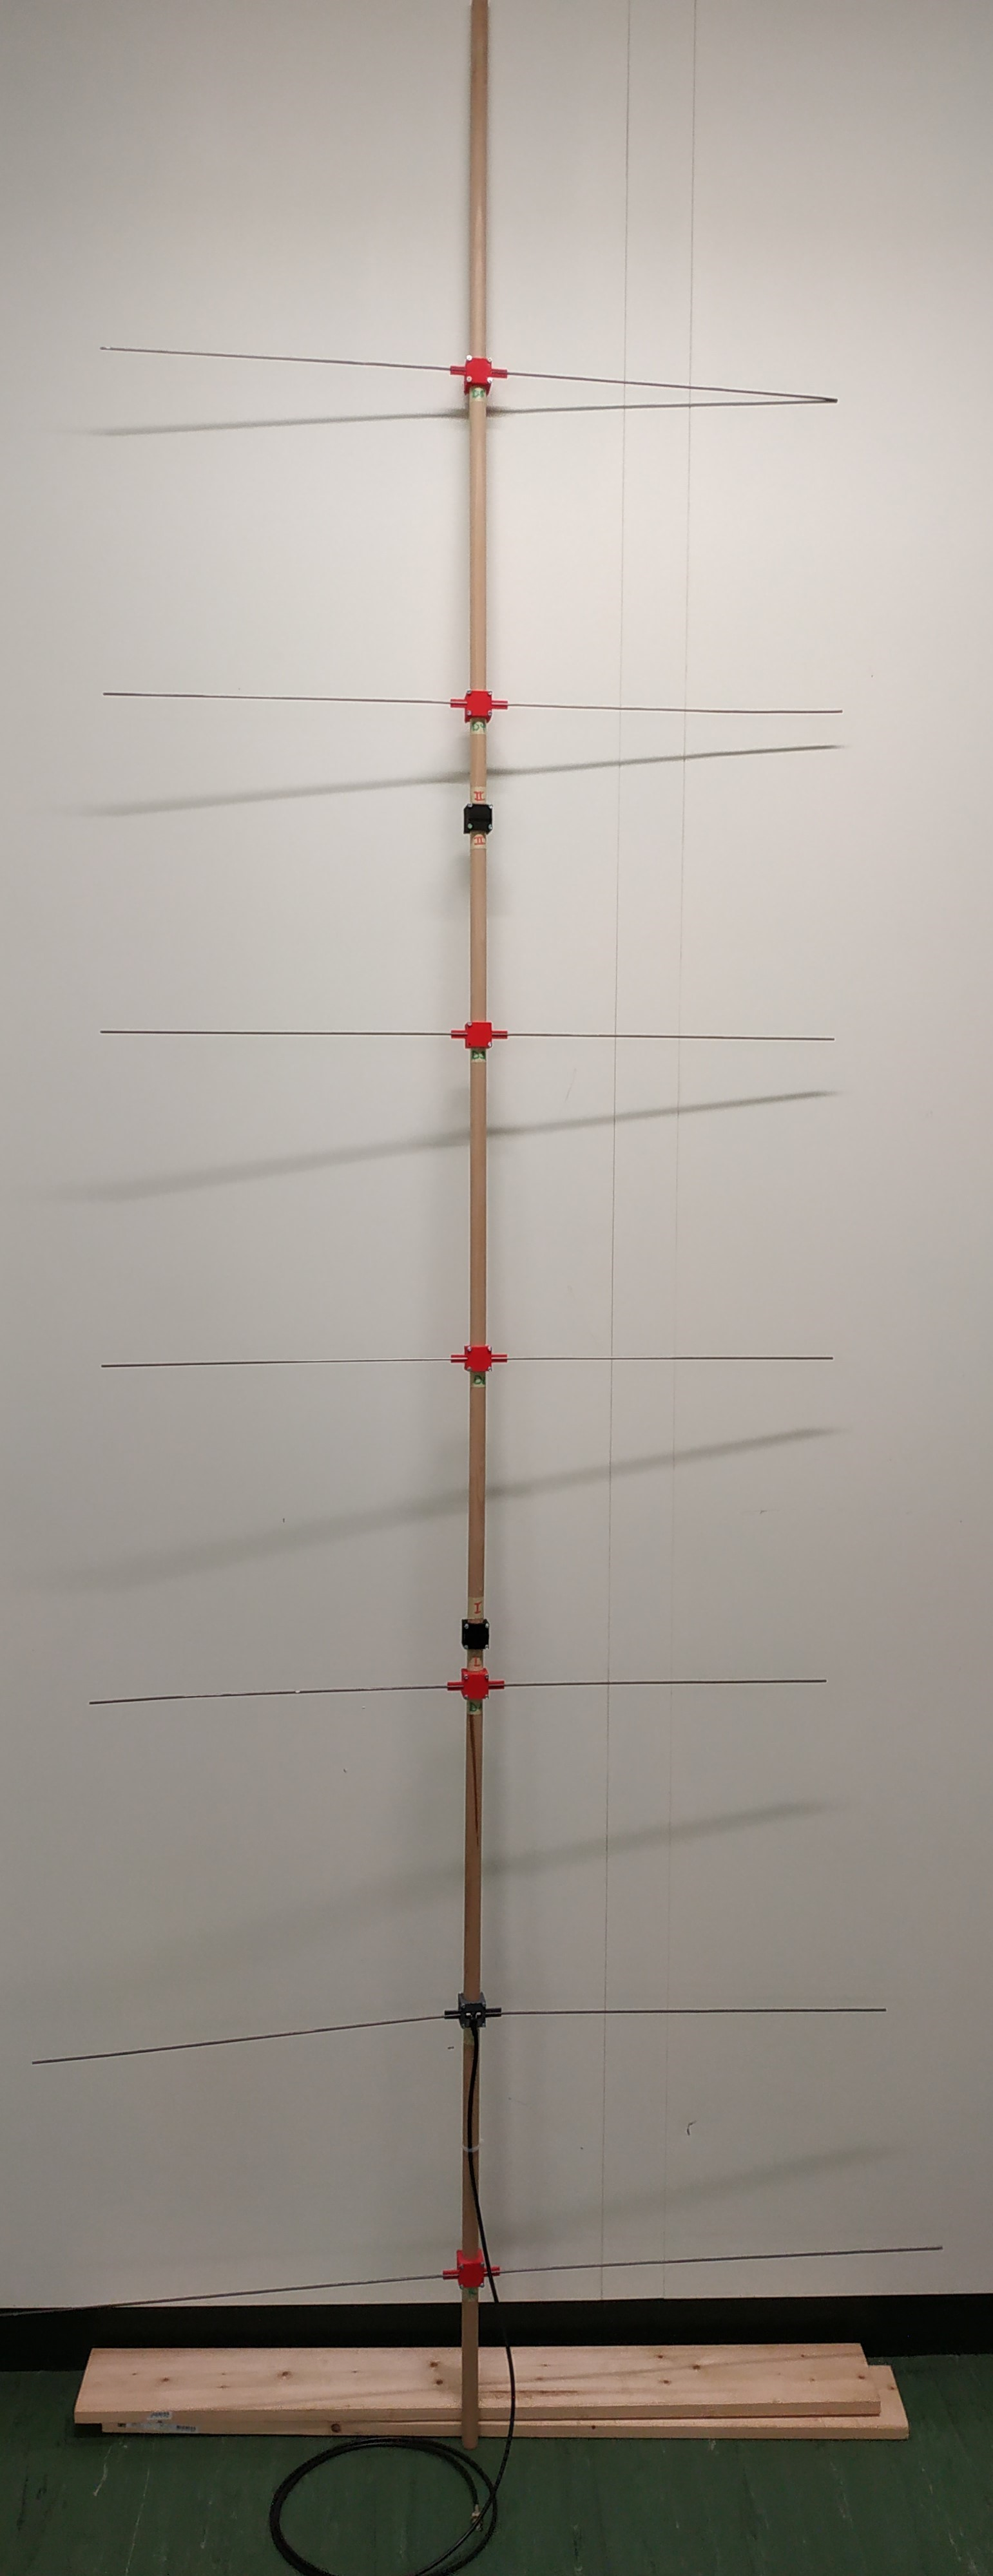
\includegraphics[width=0.28\linewidth]{yagi_eigenbau}
\end{figure}
\vfill

{
\renewcommand\arraystretch{2}
\begin{center}
\begin{tabular}{>{\bf}p{4cm} l}
Universität                &    Fachhochschule Nordwestschweiz\\
Studiengang                &    Elektro- und Informationstechnik\\
Autor   		               & 	  Simon Zoller, Thomas Frei\\
Betreuer                   &    Christoph Wildfeuer und Peter Niklaus\\
\end{tabular}
\end{center}
}

\clearpage

%%---ABSTRACT----------------------------------------------------------------------------
\selectlanguage{ngerman}				%ngerman or english
\thispagestyle{empty}
\include{sections/abstract}

%%---TABLE OF CONTENTS-------------------------------------------------------------------
\pagenumbering{Roman}
\selectlanguage{ngerman}				%ngerman or english
\tableofcontents
\clearpage

%%---TEXT--------------------------------------------------------------------------------
\pagenumbering{arabic}
\section{Einleitung}

Ein grosses Thema der Hochfrequenztechnik sind Antennen. Generell können Antennen als Leiter angesehen werden, welche sich identisch zur Leitungstheorie verhalten. Jedoch gibt es viele verschiedene Ausführungen mit unterschiedlichsten Eigenschaften. Dieser Bericht ist als Weiterführung zu dem hf1-Bericht gedacht, bei welchem viele Antennen mit \textit{CST Studio Suite} simuliert wurden. Der hf2-Bericht spezialisiert sich auf Yagi-Antennen. Neben der theoretischen Arbeit soll selber eine Yagi-Antenne für \SI{144.125}{MHz} konstruiert und gebaut werden. Hierfür wurde zuerst die Theorie erarbeitet. Mit den berechneten Werten für die Yagi-Anntene werden Simulationen mit dem Programm \textit{CST Studio Suite} durchgeführt, welche sich vor allem auf das Strahlungsdiagramm der Antenne beziehen. Als Abschluss wird die Antenne im Labor ausgemessen und verifiziert.
\section{Theorie}
Als erstes wird die Yagi-Uda-Antenne beschrieben. In einem zweiten Teil wird deren Strahlungsdiagramm betrachtet um die Abstrahlung zu verstehen. Zum Schluss soll die benötigte Theorie zur Impedanzanpassung und Wellenunterdrückung erarbeitet werden, da diese beim Antennenbau wichtig ist.

\subsection{Yagi-Uda-Antenne}\label{sec:Yagi}
Die Yagi-Uda-Antenne stammt aus Japan. 1926 erfanden Shintaro Uda und Hidetsugu Yagi die Antenne. Etwas später veröffentlichte Yagi den ersten englischen Artikel. Aus diesem Grund wir heute oft die Antenne nur noch seinem Namen in Verbindung gebracht. Ein typisches Beispiel für die Verwendung einer Yagi-Antenne ist der Fernsehrundfunkempfang. Hierfür wird die Antenne für eine Frequenz von einigen 100MHz ausgelegt.

Zur Erhöhung der Richtwirkung kann sowohl Reflektor- als auch Direktordipole an einen primär erregten Dipol angebracht werden. Oft wird eine ganze Reihe von Direktoren, bis zu 20 Stück, benutzt. Jedoch beschränkt manch sich meist auf einen Reflektor. Zur Minderung der unerwünschten Rückstrahlung baut man höchstens noch mit weiteren Stäben den Reflektor zu einer reflektierenden Wand aus.

In der Praxis werden als Reflektoren meist Halbwellendipole verwendet. Der aktive gespeiste Dipol wird etwa 6\% kürzer ausgeführt. In der Direktorreihe wird jeder Nachfolger ca. 1\% kürzer als sein Vorgänger ausgelegt. Die Elementabstände liegen um 0,3$ \lambda $. Alle Strahler sind in ihrer Mitte auf einem Trägerstab befestigt. Durch die Strahlungskopplung, welche mit zunehmendem Abstand schwächer wird, werden die passiven Dipole zum Mitschwingen angeregt. Die unterschiedlichen Längen der Elemente führen zu unterschiedlichen Phasenverschiebungen zwischen einfallender und abgestrahlter Welle. Diese Phasenverschiebung sowie der Abstand der Elemente werden so dimensioniert, dass es in Hauptstrahlrichtung zu einer konstruktiven Überlagerung der Teilwellen und damit einer starken Abstrahlung kommt. weiter die Elemente vom aktiven Dipol entfernst sind, desto weniger tragen sie zur Abstrahlung bei. Deshalb ist der erzielbare Gewinn einer Yagi-Antenne beschränkt. Wenn die Antennenlänge L auf einen Wert im Bereich $ 0.5\leq L/\lambda_{0} \leq 7$ verdoppelt wird, steigt der Gewinn nur um 2.2dB und nicht um 3dB.
\begin{figure}[H]
	\centering
	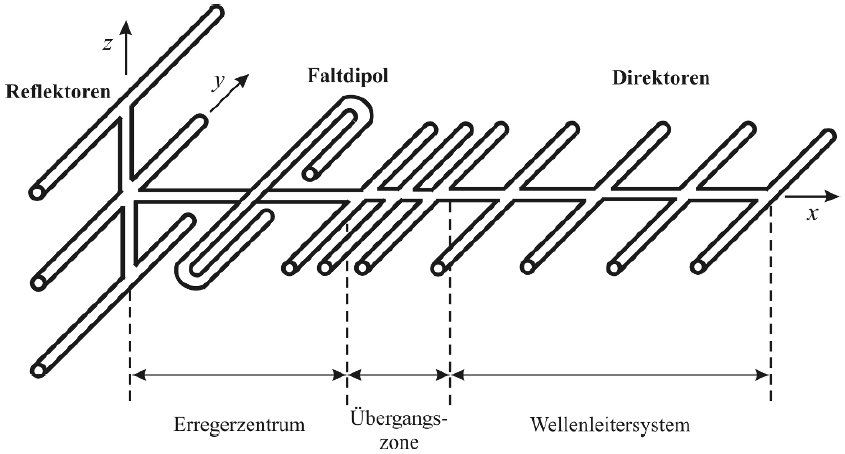
\includegraphics[width=0.8\linewidth]{yagi_antenne}
	\caption{Aufbau einer Yagi-Antenne mit einem aktiv gespeisten Faltdipol und parasitären Strahlerelementen.}\label{fig:yagi}
\end{figure}
Wie man aus der Abbildung \ref{fig:yagi} erkennen kann, lässt sich die Yagi-Antenne in drei Wirkungszonen unterteilen. Diese sind das Erregerzentrum, die Übergangszone und das Wellenleitersystem. 
\paragraph{Erregerzentrum}
Im Erregerzentrum wird die Bandbreite und der Eingangswiderstand der ganzen Antenne bestimmt. Durch die parasitären Elemente wird der Dipol stärker belastet. Deshalb wird der Strahlungswiderstand niederohmiger. Um dem entgegenzuwirken wird meistens ein Faltdipol verwendet, da er gegenüber einem "gestreckten" $\lambda/2 $-Dipol den Vorteil grösserer Breitbandigkeit und etwa viermal höheren Eingangswiderstand besitzt. Als Speiseleitung wird eine Flachbandleitung mit $ Z_{L} \approx 240\Omega $ an den Dipol angeschlossen. Der Reflektor gehört auch zum Erregerzentrum. Er kann mit zusätzlichen Stäben zu einer reflektierenden Wand erweitert werden.
\paragraph{Übergangszone}
Dieser Bereich besteht aus mehreren Direktoren. Sie dienen zur optimalen Anpassung der Strahlung des Erregerzenstrums an das folgende Wellenleitersystem.
\paragraph{Wellenleitersystem}
Mit diesem System wird die Strahlungscharakteristik der Antenne bestimmt. Es wird aus mehreren Direktoren gebildet.

\subsection{Strahlungsdiagramm}\label{sec:Strahlungsdiagramm}

Das Strahlungsdiagramm wird genutzt um  graphisch die Richtcharakteristik einer Antenne darzustellen. Das Diagramm gibt Informationen über die Feldstärkeverteilung von der Antenne in grosser Distanz. In der Abbildung \ref*{fig:richtdiagram} ist das Strahlungsdiagramm einer Yagi-Antenne dargestellt. Die Hauptstahlrichtung der Antenne breitet sich zur Richtung des Direktors aus. 

\begin{figure}[H]
	\centering
	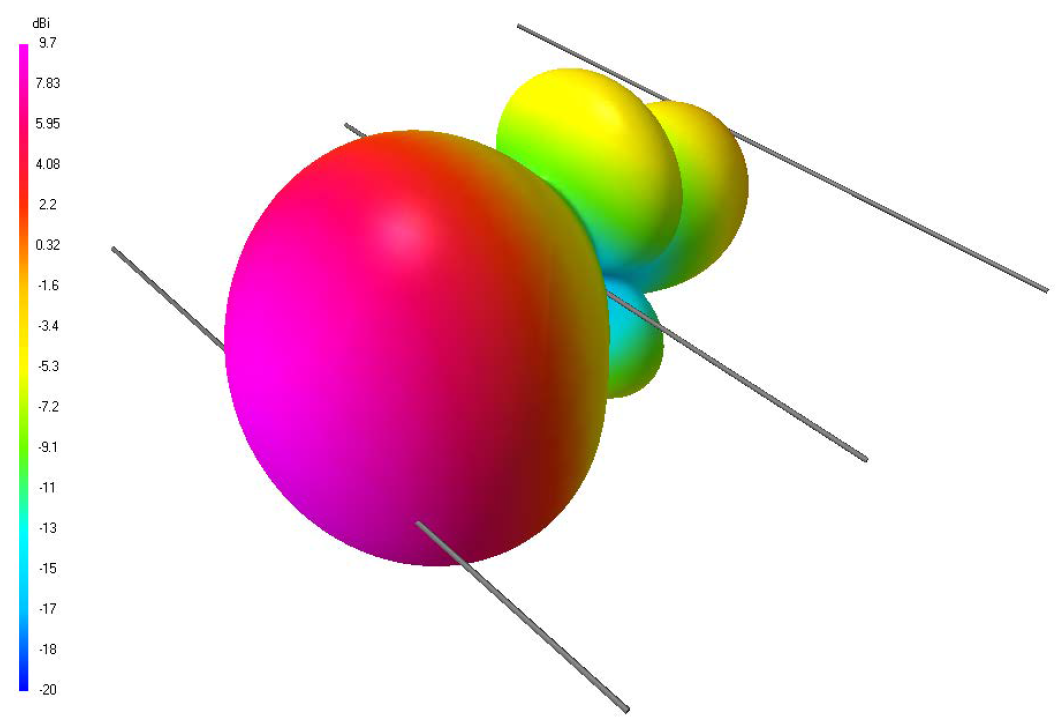
\includegraphics[width=0.8\linewidth]{yagi_richtdiagram}
	\caption{Strahlungsdiagramm einer Yagi-Antenne mit einem Direktor.}\label{fig:richtdiagram}
\end{figure}

\subsection{Impedanzanpassung ev. Flusspunktimpedanz}\label{sec:Impedanzanpassung}


\subsection{Mantelwellenunterdrückung}\label{sec:Mantelwellenunterdrückung}
\section{Berechnung}
In diesem Kapitel wird anhand der Abbildung \ref{fig:berechnung} die Abstände zwischen den Elementen sowie die Länge des Dipols, des Reflektor und den Direktoren berechnet. Die Yagi-Antenne soll für eine Frequenz von 144MHz ausgelegt werden. Diese Frequenz entspricht dem 2-Meter-Band, welches von den Amateurfunker für eine Erde-Mond-Erde-Übertragung genutzt wird. 

\begin{figure}[H]
	\centering
	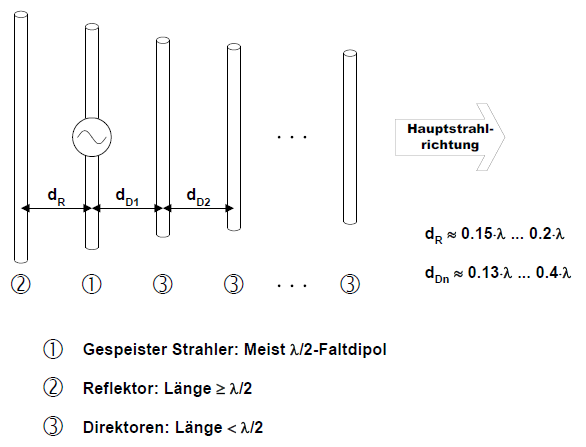
\includegraphics[width=0.9\linewidth]{yagi_berechnung}
	\caption{Aufbau einer Yagi-Antenne mit Dimensionsangaben.}\label{fig:berechnung}
\end{figure}

Die Antenne soll aus einem Reflektor einem Dipol und fünf Direktoren bestehen. Die benötigten Elemente werden in dem nachfolgenden Teil berechnet.

Die Wellenlänge $ \lambda $ für 144MHz berechnet sich wie folgt:
\begin{equation}
\lambda=\frac{c}{f_{0}}=\frac{\SI{300e06}{m/s}}{
\SI{144}{MHz}} = \SI{2.08}{m}
\end{equation}

Die Länge des Reflektor $ l_{R} $ berechnet sich wie folgt:
\begin{equation}
l_{R}\geq\frac{\lambda}{2}=\frac{\SI{2.08}{m}}{
	2} = \SI{1.04}{m} \Rightarrow \SI{1.2}{m}
\end{equation}

Die Länge des Dipols $ l_{S} $ berechnet sich wie folgt:
\begin{equation}
l_{S}=\frac{\lambda}{2}=\frac{\SI{2.08}{m}}{
	2} = \SI{1.04}{m}
\end{equation}

Die Länge der Direktoren $ l_{Dn} $ berechnet sich wie folgt:
\begin{equation}
l_{Dn}\leq\frac{\lambda}{2}=\frac{\SI{2.08}{m}}{
	2} = \SI{1.04}{m} \Rightarrow \SI{0.9}{m}
\end{equation}

Der Abstand $ d_{R} $ zwischen Reflektor und Dipol berechnet sich wie folgt:
\begin{equation}
d_{R}\approx 0.15\cdot\lambda=0.15\cdot \SI{2.08}{m}= \SI{0.312}{m}\Rightarrow \SI{0.32}{m}
\end{equation}

Der Abstand $ d_{Dn} $ zwischen Dipol und Direktor oder Direktor und Direktor berechnet sich wie folgt:
\begin{equation}
d_{Dn}\approx 0.2\cdot\lambda=0.2\cdot \SI{2.08}{m}= \SI{0.416}{m} \Rightarrow \SI{0.4}{m}
\end{equation}

Die Länge des Trägerstabs $ l_{T} $ berechnet sich wie folgt:
\begin{equation}
l_{t}=d_{R}+5\cdot d_{Dn} + Anfang = \SI{0.32}{m} + 5\cdot \SI{0.4}{m} + \SI{0.2}{m}= \SI{2.52}{m}
\end{equation}

Alle Masse sind in der Tabelle \ref{tab:bauwerte} zusammengefasst.

\begin{table}[H]
	\centering
	\begin{tabular}{>{\tt}L{6cm}|  L{3cm}} 
		\normalfont\textbf{Name} & \normalfont\textbf{Masse [m]} \\ \hline\hline 
		Wellenlänge 		&  2.08    \\ \hline
		Länge Reflektor 	&  1.2    \\ \hline
		Länge Dipol 		&  1.04    \\ \hline
		Länge Direktor  	&  0.9     \\ \hline
		Länge Trägerstab 	&  2.52    \\ \hline
		Distanz $ d_{R} $ 	&  0.32   \\ \hline
		Distanz $ d_{Dn} $ 	&  0.4    \\ \hline
	\end{tabular}
	\caption{Zusammenstellung der Längen der Elemente sowie deren Abstand zueinander.}
	\label{tab:bauwerte}
\end{table}



\section{Simulation}\label{sec:Simulationsresultate}

Für das Testen des theoretischen Aufbaus der Yagi-Antenne wurde eine Simulation mit \textit{CST Studio} durchgeführt. Somit kann vor dem Zusammenbau der Antenne dessen Funktion verifiziert werden und falsche Berechnungen überprüft werden. Dieser Abschnitt erläutert die Vorgehensweise bei der Simulation und dessen Resultate.

\subsection{Aufbau der Antenne}

Um die Antenne so realitätsnahe wie möglich simulieren zu können wurde Aluminium ($\sigma = $ \SI{3.56e+7}{S/m}) und Holz aus der Materialsbibliothek geladen. Anschliessend wurde die Antenne anhand den Parametern aus Kapitel \ref{sec:Berechnung} konstruiert. Die fertig konstruierte Antenne ist in Abbildung \ref{fig:Simulation_Yagi} zu sehen.

\begin{figure}[h!]
	\centering
	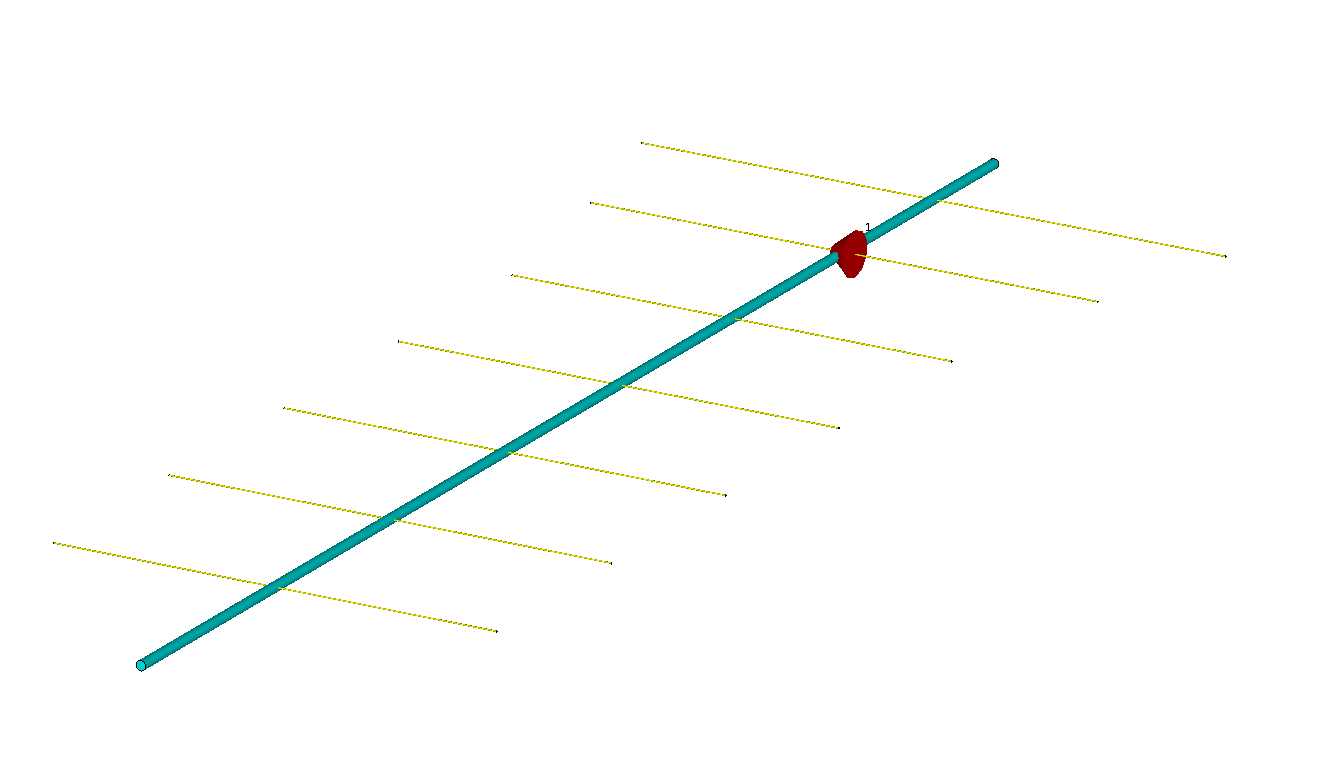
\includegraphics[width=\textwidth]{Yagi.png}
	\caption{Aufbau der Yagi-Antenne in \textit{CST Studio}.}
	\label{fig:Simulation_Yagi}
\end{figure}

\subsection{Simulationsresultate}

Für die Simulation sind für den Bericht vor allem zwei Parameter wichtig: die S-Parameter und das Fernfeld. Letzteres wurde bei \SI{144}{MHz} gemessen und ist in Abbildung \ref{fig:Simulation_Yagi_Fernfeld} zu sehen. Zur Veranschaulichung ist ein 3D-Diagramm zu sehen, wie bereits in Abbildung \ref{fig:yagi} dargestellt. Daneben befindet sich das Richtdiagramm, welches im Bericht von \textit{hf1} ausführlich beschrieben ist. Aus dem Richtdiagramm lässt sich eine Halbwertsbreite von \SI{56.0}{\degree} und eine Abstrahlstärke in Hauptrichtung von \SI{10.3}{dBi} ablesen.

 \newpage

\begin{figure}[h!]
	\centering
	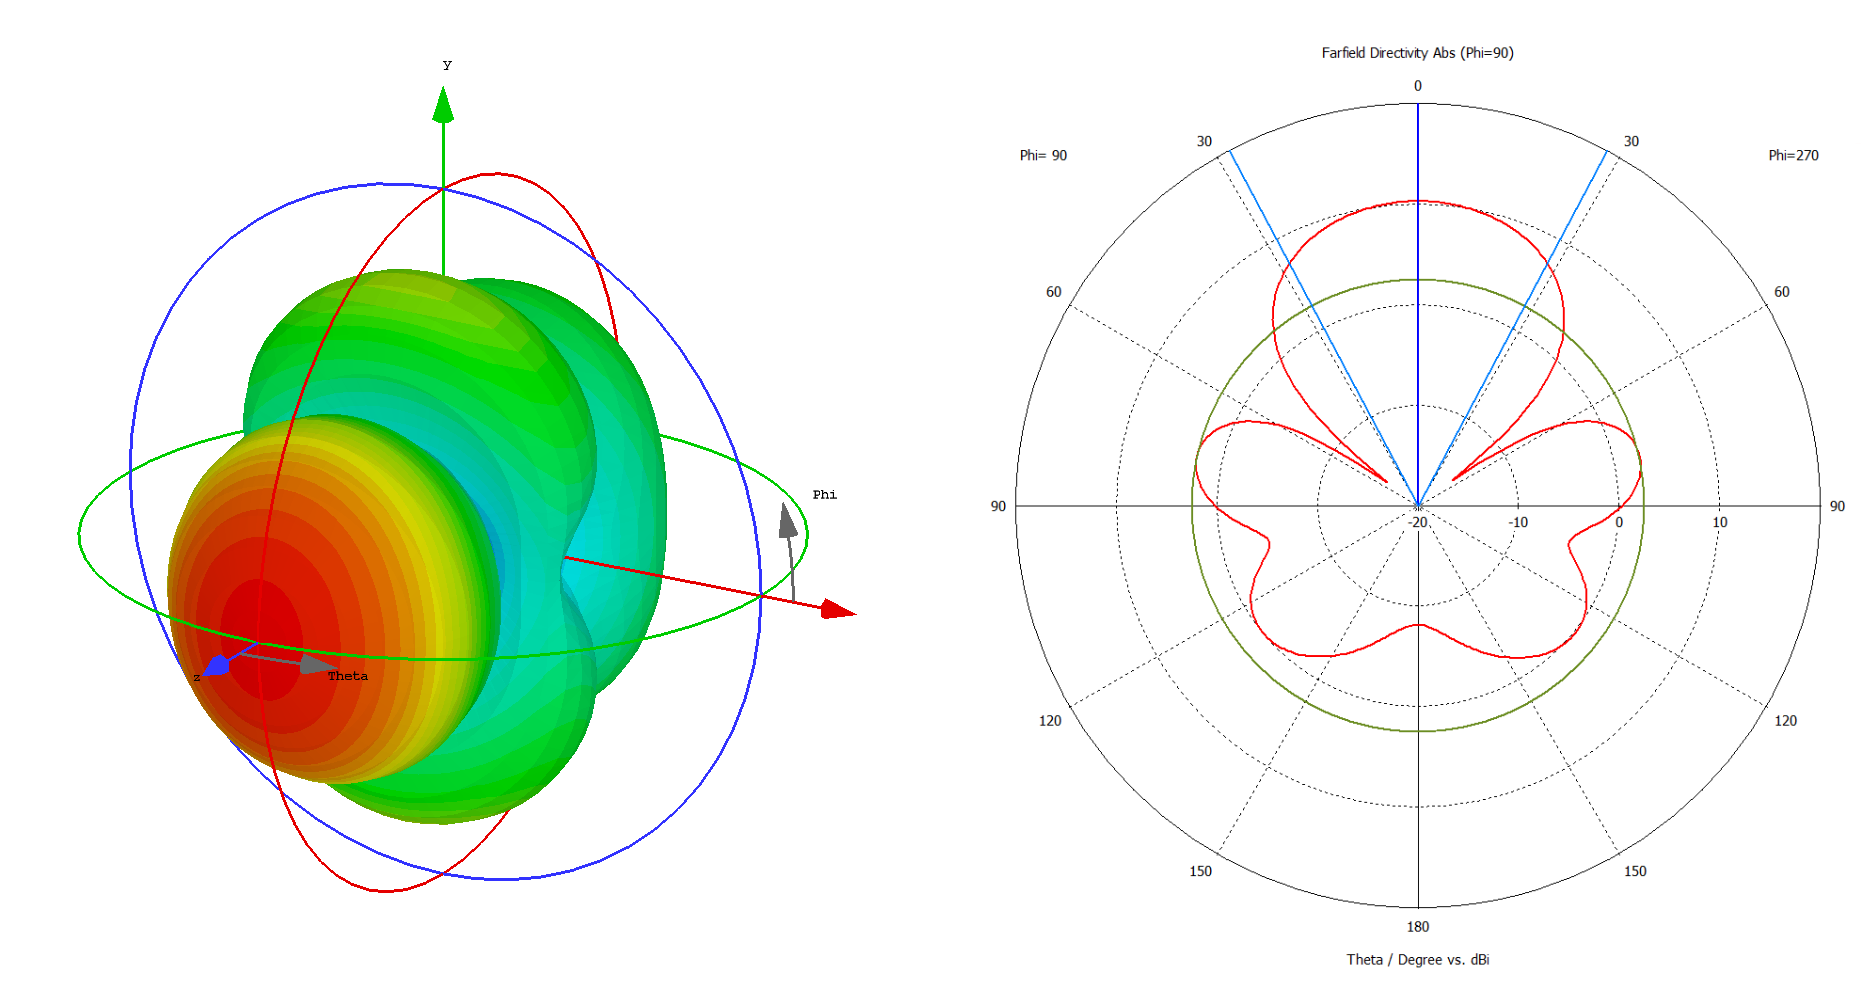
\includegraphics[width=\textwidth]{Yagi_Fernfeld.png}
	\caption{Fernfeld 3D- und Richtdiagramm der Yagi-Antenne.}
	\label{fig:Simulation_Yagi_Fernfeld}
\end{figure}

Als Vergleich wurden eine Messung mit nur zwei Direktoren durchgeführt. Die identische Simulation wurde nochmals laufen gelassen, wobei sich das 3D- und Richtdiagramm aus Abbildung \ref{fig:Simulation_Yagi_Fernfeld_2dir} ergibt. Hierbei ist bereits ersichtlich, dass die Hauptkeule viel breiter ist und sich total weniger Keulen ergeben. Die Halbwertsbreite beträgt bei dieser Antenne \SI{89.2}{\degree} und die Abstrahlstärke in Hauptrichtung \SI{7.6}{dBi}. Somit kann bestätigt werden, dass mehr Direktoren zu einer kleineren Halbwertsbreite führen und dessen Abstrahlstärke dadurch auch stärker wird.

\begin{figure}[h!]
	\centering
	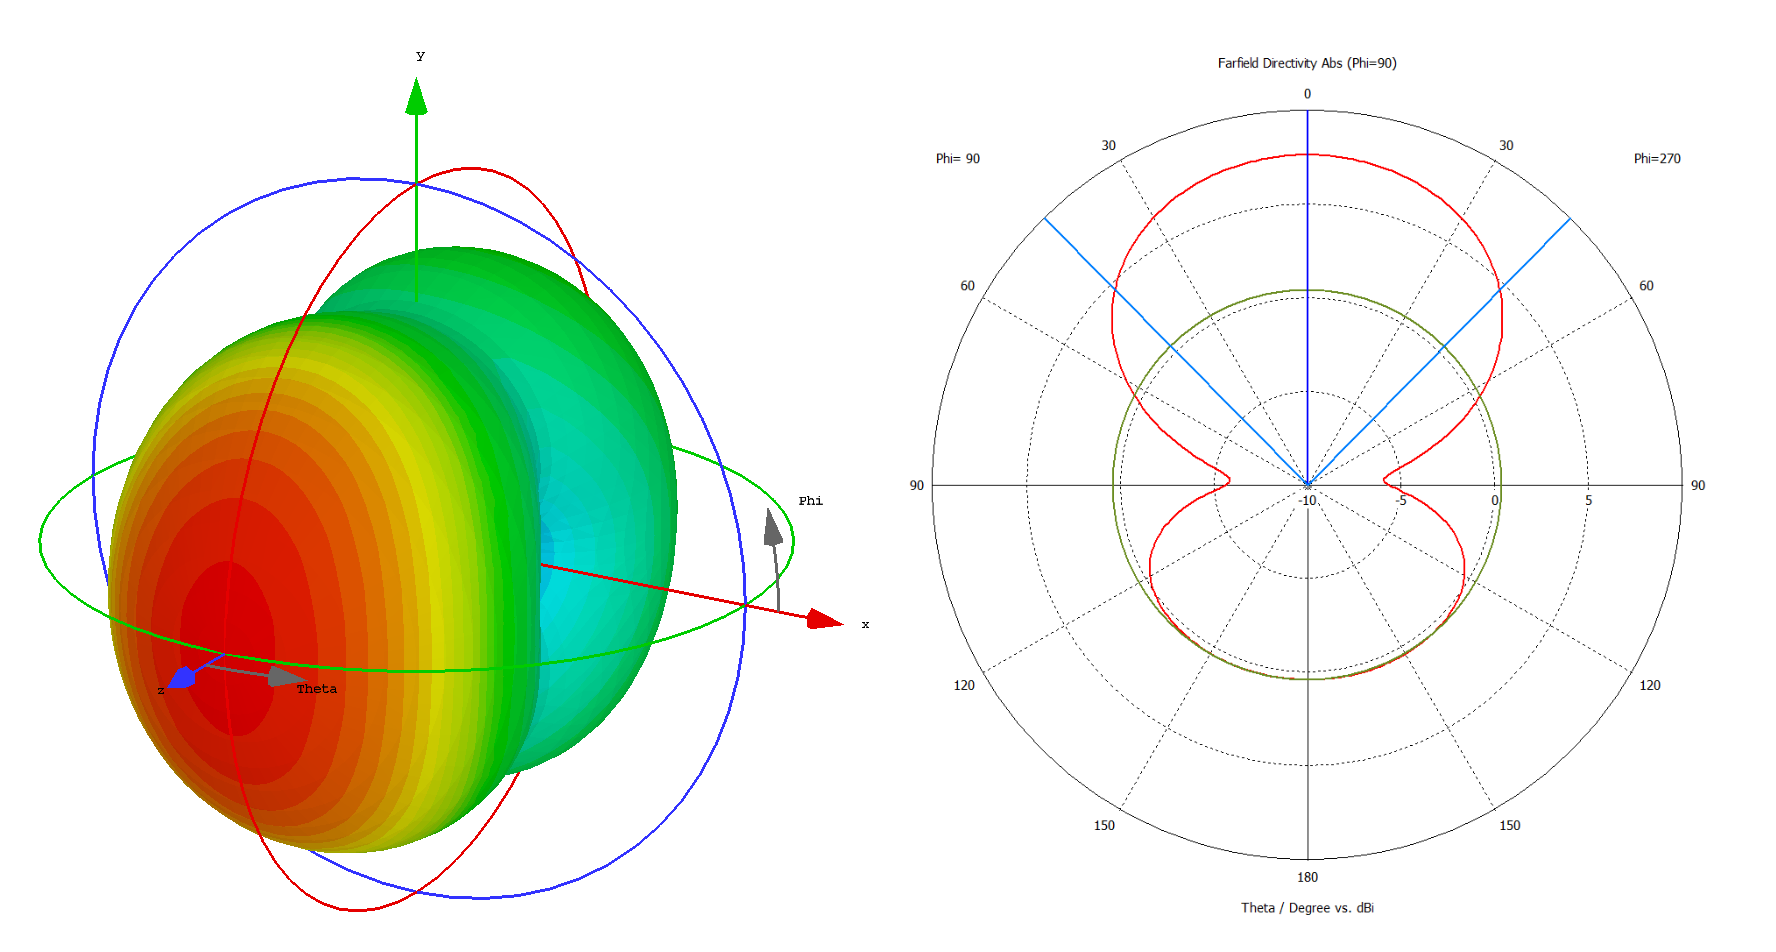
\includegraphics[width=\textwidth]{Yagi_Fernfeld_2dir.png}
	\caption{Fernfeld 3D- und Richtdiagramm der Yagi-Antenne mit nur 2 Direktoren.}
	\label{fig:Simulation_Yagi_Fernfeld_2dir}
\end{figure}

\newpage

Während die 3D-Diagramme gut sind für das Verständnis der Abstrahlung der Antenne, für den Bericht sind die Messungen bezüglich der S1,1 Parameter aussagekräftiger (und vor allem auch einfacher messbar). Diese Parameter werden anschliessend in Kapitel \ref{sec:Messung} im Labor gemessen und können als Verifikation verwendet werden. Somit wurde die Antenne mit dem \textit{Frequency Domain Solver} ausgemessen.

\begin{figure}[h!]
	\centering
	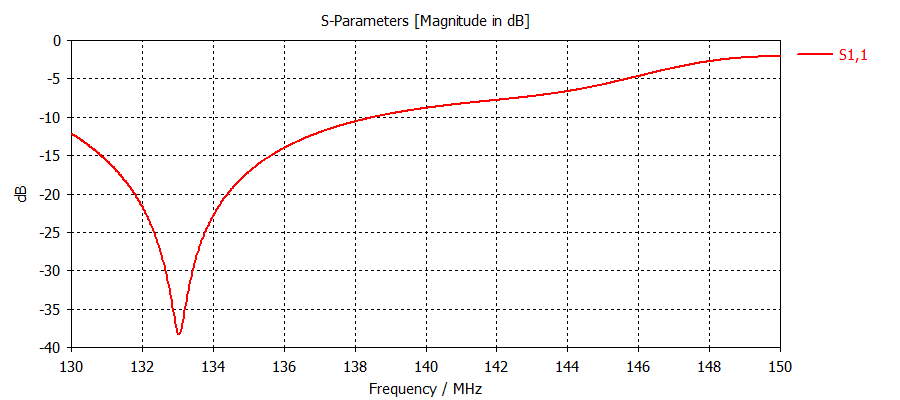
\includegraphics[width=\textwidth]{result.png}
	\caption{S1,1 Parameter der simulierten Yagi-Antenne.}
	\label{fig:Simulation_result}
\end{figure}

Abbildung \ref{fig:Simulation_result} zeigt die S1,1 Parameter der konstruierten Yagi-Antenne. Wie bereits erwähnt wurde diese für \SI{144.125}{MHz} berechnet, wobei bei der Simulation eine Grenzfrequenz von \SI{133.0}{MHz} gemessen wird. Die dabei abweichende Grenzfrequenz kann vor allem durch das Anpassen der Länge des Dipols verbessert werden. Für das bessere Verständnis der Antenne werden die für die Simulation berechneten Parameter um $\pm$ \SI{5}{cm} angepasst, womit dessen Auswirkungen auf die S1,1 Parameter dargestellt werden können.

\begin{figure}[h!]
	\centering
	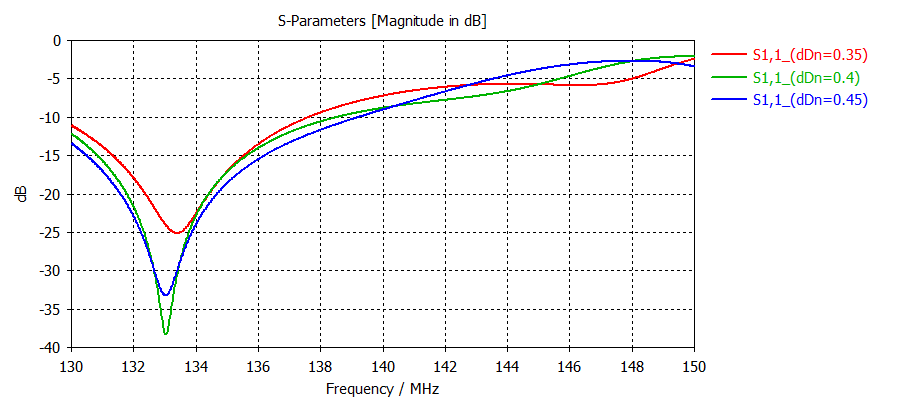
\includegraphics[width=\textwidth]{dDn.png}
	\caption{Resultat der S1,1 Parameter durch Abändern von \textit{dDn}.}
	\label{fig:Simulation_dDn}
\end{figure}

In Abbildung \ref{fig:Simulation_dDn} wird das Resultat durch verändern des Abstandes zwischen den Direktoren dargestellt. Erwartungsgemäss hat dieser Abstand nahezu keinen Einfluss auf die Grenzfrequenz, sondern nur auf den Antennengewinn. Kleine Abweichungen vom berechneten Wert können dabei bereits eine Verschlechterung von \SI{15}{dB} ausmachen (dies liegt jedoch auch daran, dass alle 5 Direktoren dabei voneinander um \SI{5}{cm} verschoben werden, weshalb der letzte Direktor ganze \SI{25}{cm} weiter hinten liegt).

\begin{figure}[h!]
	\centering
	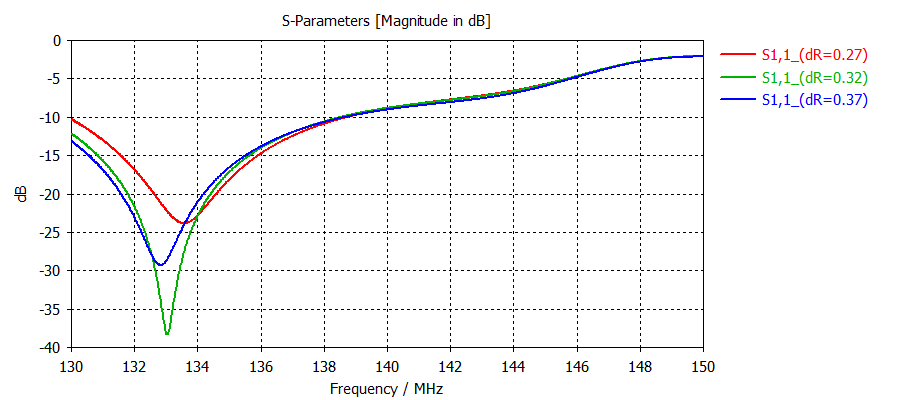
\includegraphics[width=\textwidth]{dR.png}
	\caption{S1,1 Parameter mit sich änderndem Abstand des Reflektors zum Dipol.}
	\label{fig:Simulation_dR}
\end{figure}

Auch ein Abändern des Abstandes des Reflektors zum Dipol hat nur einen minimen Einfluss auf die Grenzfrequenz. Dies ist der Abbildung \ref{fig:Simulation_dR} zu entnehmen. Dabei haben die kleinen Veränderungen nahezu das selbe Ausmass wie bei den Direktorenabständen in Abbildung \ref{fig:Simulation_dDn}. Das Verhalten der S1,1 Parameter entfernt der Grenzfrequenz ist jedoch nahezu identisch.

\begin{figure}[h!]
	\centering
	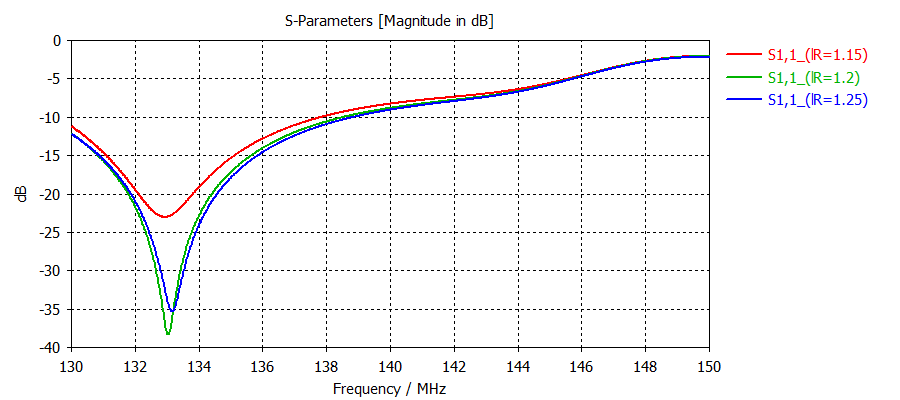
\includegraphics[width=\textwidth]{lR.png}
	\caption{Resultat durch Abändern der Reflektorlänge.}
	\label{fig:Simulation_lR}
\end{figure}

Wie im Kapitel \ref{sec:Berechnung} beschrieben soll die Länge des Reflektors mindestens eine halbe Wellenlänge betragen. Dieser Wert wurde grosszügig gerundet, wobei Abbildung \ref{fig:Simulation_lR} zu entnehmen ist, dass zu kleine Werte für die Reflektorlänge dem Antennengewinn viel mehr schaden als zu grosse Werte. Daher lohnt es sich, die Yagi-Antenne eher zu überdimensioneren anstelle von zu knappen Werten, damit der Antennengewinn nicht zu schwach ist. Jedoch muss dabei auch beachtet werden, dass ein zu langer Reflektor wiederum den Antennengewinn verschlechtern kann. Daher muss bei einem genauen Design ein Optimum gefunden werden.

\begin{figure}[h!]
	\centering
	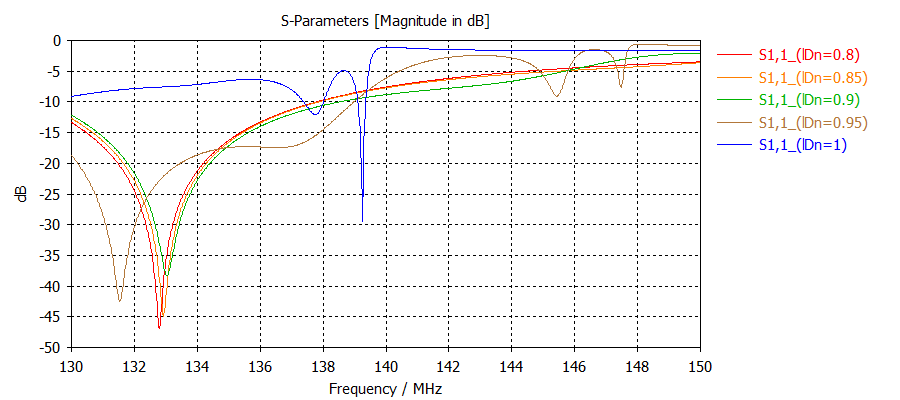
\includegraphics[width=\textwidth]{lDn.png}
	\caption{Einfluss der Direktorenlänge auf die S1,1 Parameter.}
	\label{fig:Simulation_lDn}
\end{figure}

Der Einfluss der Direktorenlänge ist in Abbildung \ref{fig:Simulation_lDn} zu sehen. Diese soll, wie in den Berechnungen beschrieben, weniger als eine halbe Wellenlänge betragen. Dabei scheinen zu knapp dimensionerte Werte sehr merkwürdige Resultate abzuliefern, weshalb bei dieser Simulation zwei zusätzliche Messungen durchgeführt wurden (eine Direktorenlänge von \SI{1}{m} beträgt weniger als eine halbe Wellenlänge, liefert jedoch schon zu schlechte Resultate). Bei kürzeren Direktoren wird nicht viel Antennengewinn aufgegeben, während für lange Werte die Grenzfrequenz stark verschoben wird (für die Messung mit dem längsten Reflektor liegt diese ausserhalb des gemessenen Bereiches). Daher lohnt es sich, diese eher zu kurz zu wählen.

\begin{figure}[h!]
	\centering
	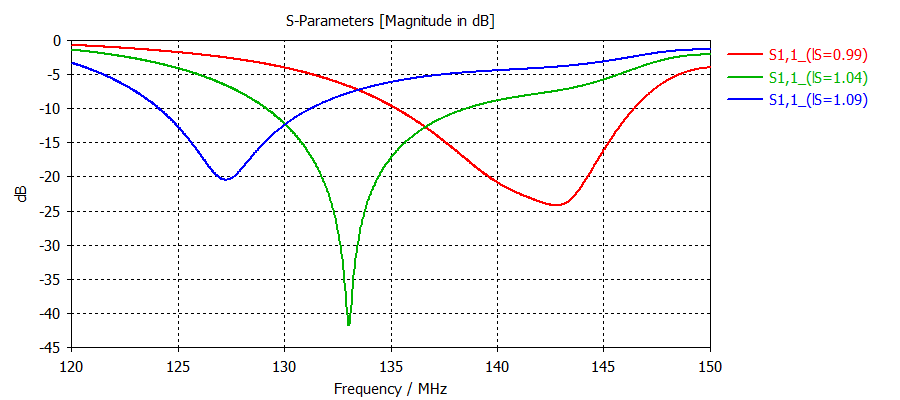
\includegraphics[width=\textwidth]{lS.png}
	\caption{Verhalten der S1,1 Parameter bei Abändern der Länge des Strahlers.}
	\label{fig:Simulation_lS}
\end{figure}

Abbildung \ref{fig:Simulation_lS} zeigt wie sich die Grenzfrequenz beim Abändern der Strahlerlänge verhält. Idealerweise beträgt diese Länge exakt eine halbe Wellenlänge, jedoch hat die Simulation gezeigt, dass die Grenzfrequenz der berechneten Antenne ungefähr \SI{10}{MHz} zu tief liegt. Diese Simulation zeigt jedoch, dass die Dimensionerung für die berechnete Antenne sich am Besten verhält im Gegensatz zu den anderen zwei Simulationen. Für kürzere oder längere Strahler kann die Grenzfrequenz im Gegensatz zu den vorherigen Messungen am effektivsten verschoben werden, jedoch leidet der Antennengewinn stark darunter.

\begin{figure}[h!]
	\centering
	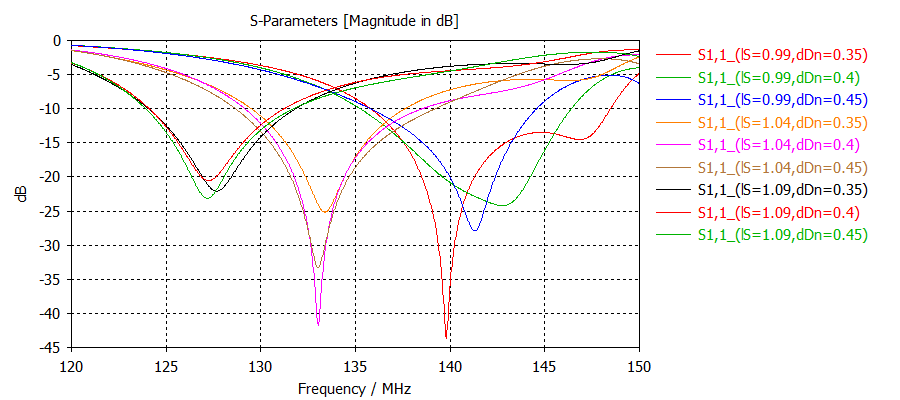
\includegraphics[width=\textwidth]{lS_dDn.png}
	\caption{Einfluss der Abänderung der Strahlerlänge und des Direktorenabstandes auf die S1,1 Parameter.}
	\label{fig:Simulation_lS_dDn}
\end{figure}

Anhand der vorherigen Simulation kann angenommen werden, dass bloss ein Abändern der Strahlerlänge nicht ausreicht. Deshalb wurde als Beispiel eine weitere Grösse angepasst. In Abbildung \ref{fig:Simulation_lS_dDn} sind die S1,1 Parameter zu sehen bei Veränderng der Strahlerlänge und der Direktorenabstände. Dabei wird zum Beispiel aufgezeigt, dass bei einem kürzeren Strahler druch das Anpassen der Direktorenabstände der Antennengewinn stark verbessert werden kann. Somit wurde durch die Simulation ein Parameterset gefunden, für welches die Antenne bie \SI{140}{MHz} sehr gute Eigenschaften besitzt. Dieses Verfahren könnte weiter verwendet werden, um ein Optimum bei \SI{144}{MHz} zu erreichen, was bei 5 veränderbaren Grössen relativ kompliziert werden kann. Da jedoch ein Grossteil der Simulationen bereits optimale Eigenschaften bei \SI{133}{MHz} aufweisen, wurden für den Bau der Antenne die bereits berechneten Werte verwendet.

\section{Aufbau}\label{sec:aufbau}

In der Abbildung \ref{fig:aufbau} ist die zusammengebaute Yagi-Uda-Antenne dargestellt. Die wichtigsten Bestandteile der Antenne sind die 3D-Elemente, die Aluminiumstäbe, das Rundholz und die Speisung des Dipols. Alle benötigten Bauteile sind in der Tabelle \ref*{tab:materialliste} aufgeführt. Jedes dieser Bestandteilen ist mit einer Nummer versehen, welche sich in der Abbildung beim passenden Element befindet. Die 3D-Elemente und der Aufbau des Dipols werden später noch genauer erklärt.

\begin{figure}[H]
	\centering
	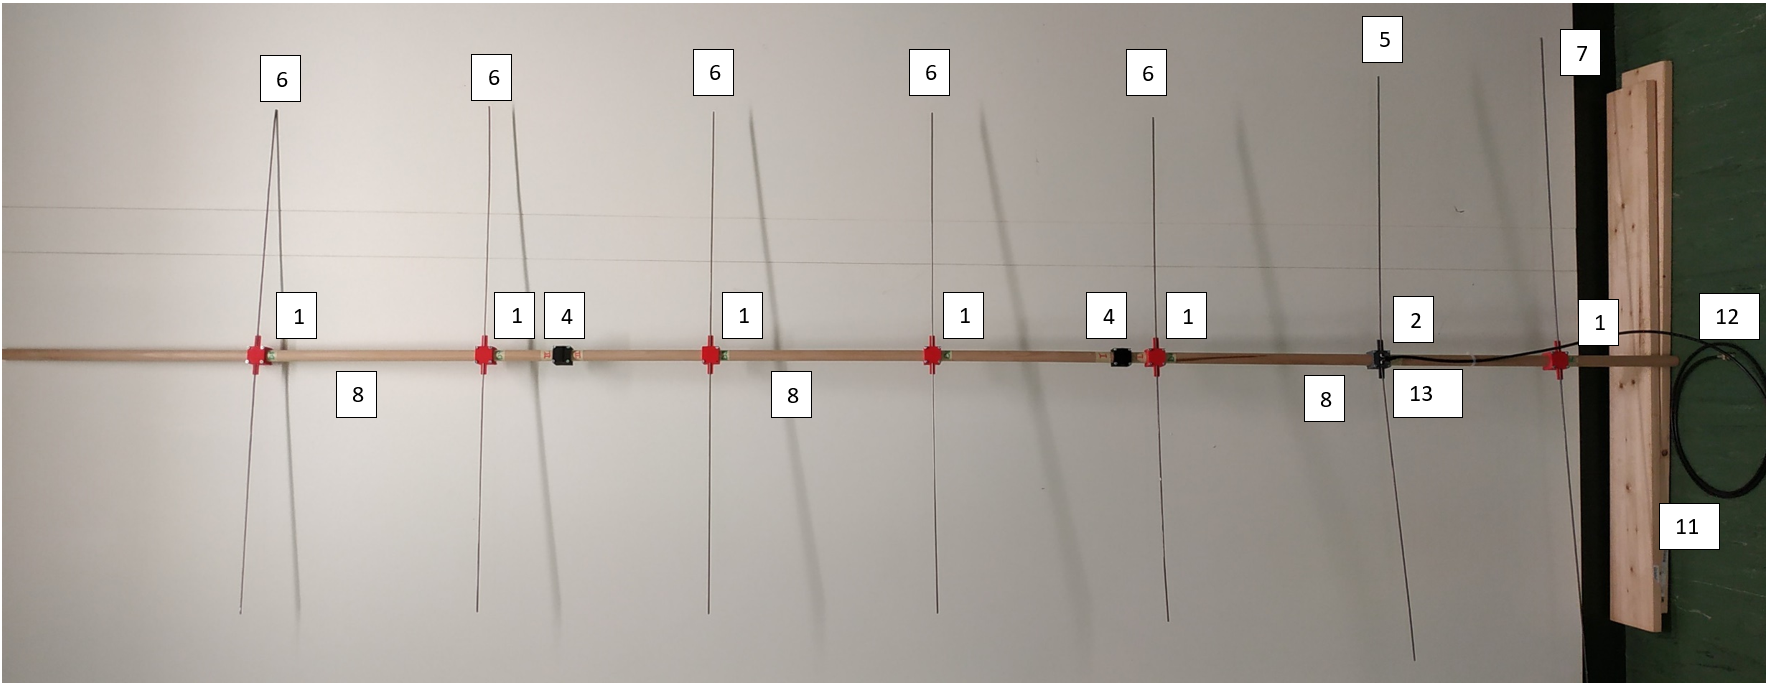
\includegraphics[width=0.9\linewidth]{aufbau}
	\caption{Aufbau eigener Yagi-Antenne mit nummerierten Bauteilen}\label{fig:aufbau}
\end{figure}

\begin{table}[H]
	\centering
	\begin{tabular}{>{\tt}C{1.7cm}| L{6.5cm}| L{3.6cm}| C{1.5cm}}
		\normalfont\textbf{Nummer} & \normalfont\textbf{Bauteil} & \normalfont\textbf{Hersteller} & \normalfont\textbf{Anzahl} \\ \hline\hline
		1	&	3D-Element Direktor/Reflektor 	& Eigenkonstruktion	& 6    \\ \hline
		2	&	3D-Element Dipol 				& Eigenkonstruktion	& 1    \\ \hline
		3	&	3D-Element Unten 				& Eigenkonstruktion	& 7    \\ \hline
		4	&	3D-Element Halterung 			& Eigenkonstruktion	& 2    \\ \hline
		5	&	Aluminiumstab $\oslash \SI{2}{mm}$ Dipol 			& FHNW Werkstat		& 1    \\ \hline
		6	&	Aluminiumstab $\oslash \SI{2}{mm}$ Direktor 		& FHNW Werkstat		& 5    \\ \hline
		7	&	Aluminiumstab $\oslash \SI{2}{mm}$ Reflektor 		& FHNW Werkstat 	& 1    \\ \hline
		8	&	Holzrundstab  $\oslash \SI{20}{mm}$, L=$\SI{1}{m}$					& Jumbo			 	& 3    \\ \hline
		9	&	M3 Impusschrauben  				& Institut ISE		& 36    \\ \hline
		10	&	M3 Mutern  						& Institut ISE 		& 36    \\ \hline
		11	&	Kabel 							& Institut ISE 		& 1    \\ \hline
		12	&	Stecker	  						& Institut ISE 		& 1    \\ \hline
		13	&	Kabelschuh	  					& Institut EA		& 2    \\ \hline
	\end{tabular}
	\caption{Zusammenstellung aller verwendeten Bauteilen.}
	\label{tab:materialliste}
\end{table}

Die Halterung für den Dipol, den Reflektor und die Direktoren sind mit einem 3D-Drucker hergestellt worden. Die Zeichnungen sind im Autodesk Fusion 360 konstruiert worden und danach mit dem Ultimaker 2+ gedruckt. Die Elemente sind in der Abbildung \ref*{fig:3D-Elemente} dargestellt.\\

Das spezielle der Konstruktion für die Halterung für den Dipol (Bild a) ist, dass sie Platz bietet um das Koaxialkabel anzuschliessen sowie die beiden Aluminiumstäbe, welche den Dipol bilden in der Mitte trennt.\\
Die Halterung für den Direktor/Reflektor (Bild b) ist so konstruiert, dass der Aluminiumstab sehr einfach durch die Öffnung hindurchgeschoben und mit Leim fixiert werden kann. \\
Mit dem Gegenstück der Halterung (Bild c), vier Impusschrauben und dem Oberteil (Bild a,b) kann das Element auf dem Trägerstab montiert werden. Die drei Trägerstäbe werden mit zwei Gegenstücke zusammengebaut. Nun können die Distanzen zwischen den Elementen ganz einfach angepasst werden durch leichtes lösen der Schrauben.

\begin{figure}[H]
	\centering
	\subfloat[Halterung für den Dipol]{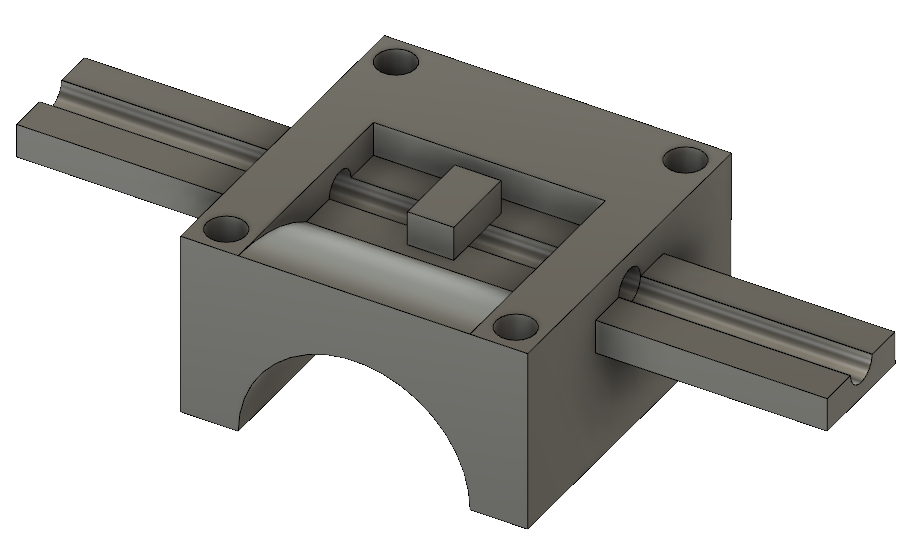
\includegraphics[width=0.4\linewidth]{oben_dipol}}\qquad
	\subfloat[Halterung für die parasitären Element]{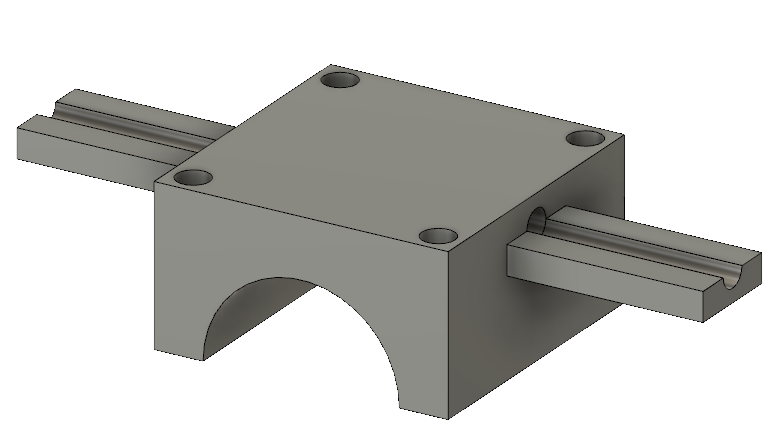
\includegraphics[width=0.4\linewidth]{oben_direktor}}\qquad
	\subfloat[Gegenstück der Halterungen]{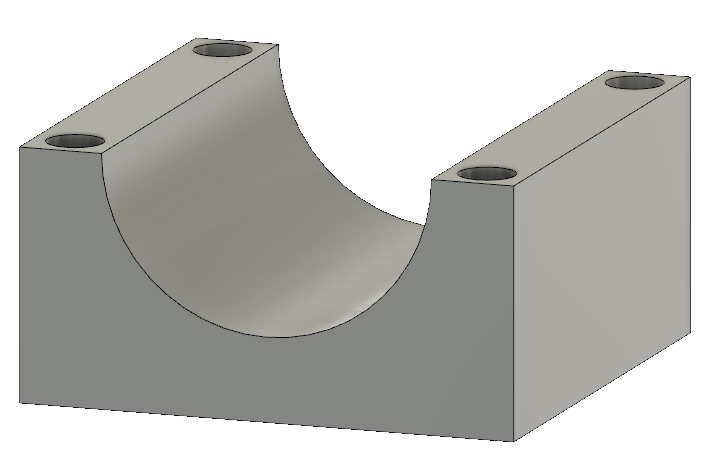
\includegraphics[width=0.3\linewidth]{unten}}
	\caption{Zeichnungen der 3D-gedruckten Elemente }
	\label{fig:3D-Elemente}
\end{figure}

In der Abbildung \ref*{fig:aufbau_dipol} ist der Aufbau des Dipols dargestellt. Der Leiter des Koaxialkabels ist am einten Teil und er Schirm an dem anderen Teil des Diplos angebracht. Die Befestigung wurde mit einem Kabelschuh realisiert. Dafür wurde bei dem Aluminiumstab ein Aussengewinde gedreht. Zum Schutz wurde das ganze mit einem Schrumpfschlauch versehen.

\begin{figure}[H]
	\centering
	\includegraphics[width=0.45\linewidth]{dipol}
	\caption{Aufbau des Dipols der Yagi-Antenne}\label{fig:aufbau_dipol}
\end{figure}

\section{Messung}




\section{Fazit}\label{sec:Fazit}

Als Fazit kann gezogen werden dass die Simulationen und der Bau der Yagi-Antenne ein Erfolg war. Es wurde eine Grenzfrequenz von \SI{144.125}{MHz} angestrebt, wobei die Simulation und Messung mit den \SI{133}{MHz} nur leicht davon abweichen. Während den Simulationen wurde viel über das Verhalten der Antenne gelernt, wobei es sehr viel mehr zu erlernen gibt. Vor allem für eine Optimierung der Antenne würden sich noch viele Möglichkeiten bieten, da sich die Werte aus der Theorie und der Praxis um einige Prozent abweichen. Zum Beispiel könnte der Dipol verkürzt werden und mit dieser sich neu ergebender Wellenlänge die Berechnungen nochmals durchgeführt werden. Somit kann ein genaueres Erreichen der \SI{144.125}{MHz} angestrebt werden. 

Ein weiteres Erfolgserlebnis war das Empfangen von Radiosendern mit der gebauten Antenne zusammen mit einem \textit{FUNcube Dongle}. Dabei konnte das Signal klar und mit besserem Gewinn empfangen werden. Das Rauschen war dabei minimal und es konnte angemessen Musik gehört werden.

Gesamthaft war der Lerngewinn sehr hoch und zusammen mit dem Bericht aus dem \textit{hf1}-Unterricht konnte sehr viel über Antennen und Simulationen mit dem \textit{CST Studio Suite} gelernt werden.



%%---BIBLIOGRAPHY------------------------------------------------------------------------
{\sloppypar
\printbibliography[heading=bibintoc]
\label{sec:lit}
}

%%---APPENDIX----------------------------------------------------------------------------
%\include{sections/appendix}

%%---NOTES for DEBUG---------------------------------------------------------------------
\ifdraft{%Do this only if mode=draft
%%requires \usepackage{todonotes})
\newpage
\listoftodos[\section{Todo-Notes}]
\clearpage
}
{%Do this only if mode=final
}
\end{document}
